\section{Arquitectura}

\subsection{Formato de representación de música}

\todo{Repasar formalizar}

La estructura para representar la música propuesta en el proyecto está determinada por un árbol que trabaja desde el elemento más general, la canción que se va a componer, al más específico, cada una de las notas que componen dicha canción, como muestra la Figura~\ref{fig:structmusic}.\\
	
	\begin{figure}[htbp]
	\centering
	\hspace*{-0.67in}
	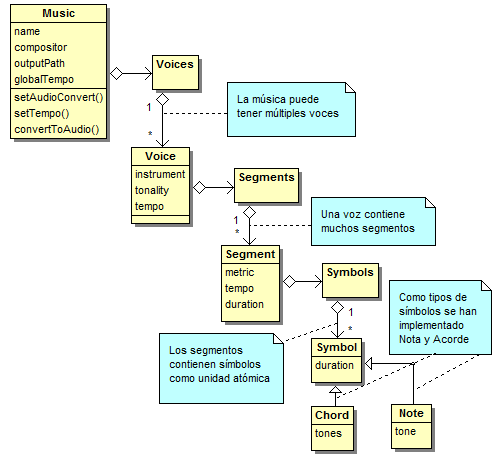
\includegraphics[scale=0.57]{graphics/musica-estructura.png}
	\caption{Estructura de la música}
	\label{fig:structmusic}
	\end{figure}


\textbf{Música}: Al nivel de la Música, trabajamos con la información relativa a toda la canción que se va a componer, por un lado está información relativa al nombre de la composición y del compositor que la ha hecho, también dispone de una serie de voces a partir de las cuales estará formada la canción y su tempo. Por último a un nivel mas cercano a la implementación permitirá elegir con que herramienta querremos crear el archivo de audio de salida.
\newline

\textbf{Voz}: Por debajo de la Música se trabaja con las Voces. Su estructura permite determinar el instrumento, la tonalidad y el tempo de cada una de las voces que componen una Música,cada una de estas voces esta compuesta de varios segmentos musicales, los cuales al ser reproducidos en el orden establecido por el compositor forman la Voz en cuestión.
\newline

\textbf{Segmento}: Estos elementos tienen la posibilidad de establecer su propia métrica, su tempo y su duración. Los segmentos a su vez están formados por una sucesión de símbolos.
\newline

\textbf{Símbolo}: Son la unidad a partir de los cuales se crean todos los elementos básicos de la música, símbolo nos permite establecer una duración para estos elementos. Actualmente el proyecto crea dos tipos de elementos a partir de símbolo:
\begin{itemize}
\item \textbf{Notas}: Estos símbolos tienen asociada una duración, determinada por el componente anterior, y un tono establecido por un número que posteriormente será interpretado con la herramienta que generará el archivo de audio.
\item \textbf{Acordes}: Los acordes están formados de la misma manera que las notas pero en lugar de tener asociado un único tono pueden tener de dos a tres tonos diferentes, en la canción esto resultará en todos los tonos sonando a la vez durante el mismo tiempo una vez generada la canción.
\end{itemize}

\subsection{Formato de representación de imágenes}

\todo{está en google docs, sólo es pasarlo a limpio}

\subsection{Sistema de análisis de Imágenes: Phic}

\todo{hacer}

\subsection{Sistema de composición algorítmica: Mu}

\todo{hacer}

\subsection{Sistema de enlace de módulos: Muphic}

\todo{hacer}

\subsubsection{Interfaz Gráfica}

El desarrollo de la interfáz gráfica se decidió realizar a través de un framework que facilitase la construcción de la misma. Qt, la herramienta que se utilizó se eligió debido a dos criterios, era multiplataforma, al igual que la aplicación, servía para trabajar con móviles, siguiendo así uno de los enfoques iniciales del proyecto que más adelante fue descartado. Además Qt trabaja con C++ como lenguaje de programación, el mismo que el núcleo de la aplicación y ofrece facilidades a la hora de integrar audio, a través de la librería Phonon, o componentes personalizados en una interfaz.\\
\todo{Este párrafo no se si abriría mejor la parte de arquitectura}
\newline
La interfáz esta compuesta de tres pestañas cada una encargada de una parte de la funcionalidad:
\newline
\\\underline{Graphic Config:}
\\En esta pestaña se encuentran todas las opciones relacionadas con el análisis de la imagen, las distintas configuraciones se transmitirán a los módulos de la aplicación a través de un documento XML que se genera cuando en la "Main Window" se le da al boton de "Analyze".
\\Los distintos componentes de esta pestaña van variando según el filtro que se seleccione, sin embargo algunos de ellos son comunes para todos los filtros:
\newline
\\\textit{Filter:} Este combo box permite seleccionar entre los distintos filtros que se pueden usar en la aplicación.
\\\textit{Noise Selection:} Con esta barra de desplazamiento se podrá elegir a partir de que tamaño, relativo al area del mayor polígono de la imagen, se ignorarán los poligonos encontrados durante el análisis de la imagen.
\\\textit{Analysis Depth:} Esta barra permite seleccionar cuanto deseamos comprimir la imagen original antes de analizarla, cuando menor sea su valor menor será el nivel de detalle obtenido y más rápido se realizará el análisis.
\\\textit{Polygon Simplification:} Esta barra permite seleccionar cuanto deseamos simplificar los poligonos obtenidos a partir de la imagen original, cuanto mayor sea su valor menos vertices tendrán los poligonos obtenidos y por lo tanto menos fiel será el resultado del análisis, sin embargo, este se realizará más rápido.
\newline
\\Según el filtro que se elija aparecerán mas componentes:
\newline
\\\todo{Rellenar esto de manera experta y didáctica}
\\\textit{Threshold} (Filtro Threshold): 
\\\textit{Hue Division} (Filtro Hue Division):
\\\textit{Threshold H} (Filtro Multiple Threshold):
\\\textit{Threshold S} (Filtro Multiple Threshold):
\\\textit{Threshold V} (Filtro Multiple Threshold):
\newline
\\\underline{Composition Config:}
\\En esta pestaña se pueden encontrar todas las opciones disponibles para el compositor musical, estás serán transmitidas a los modulos de la aplicacióncuando se pulse el boton de "Compose" en la "Main Window" a través del documento XML mencionado anteriormente.
\\Como se puede ver en la imagen adjunta, hay opciones para cuatro voces, que son aquellas con las que trabajan los compositores de la aplicación siendo, normalmente, la "Voice 1" la melodía principal, la "Voice 2" un acompañamiento, la "Voice 3" el bajo y la "Voice 4" la percusión. Las opciones disponibles son las siguientes:
\\\todo{Adjuntar imagen}
\newline
\\textit{Color System:} Hace referencia referencia a la teoría sinestésica que se utilizará como base para la relación de color-notas durante la composición musical.
\\textit{Composer:} En las cuatro voces se refiere a que compositor se utilizará para esa voz, al presionarlo se desplegarán los distintos compositores que estan disponibles para que el usuario elija el que mejor le convenga.
\\textit{Instrument:} En las cuatro voces se refiere a que instrumento se utilizará para esa voz en concreto, al presionarlo se desplegarán los instrumentos disponibles.
\\textit {Composer Mixer:} Hace referencia a que como se combinarán las cuatro voces anteriores.
\\textit{Tempo:} 
\\\todo{A rellenar con gente que sepa describirlo mejor que yo. \\También hay que repasar lo anterior}
\newline
\\{\bf Libreria Phonon}
\\Esta es una librería proporcionada por Qt para la reproducción de audio, al ser un módulo externo requiere una serie de librerias añadidas que están incluidas en el paquete de instalación de windows, sin embargo tendrán que ser instaladas en linux utilizando alguno de los gestores de software disponibles realizando una busqueda con la palabra clave: Phonon.
\\Las librerías requeridas son las siguientes: (LISTA DE LIBRERIAS)
\\En el caso de que no funcione el sistema de reproducción, se pueden encontrar los archivos de audio en la ruta especificada en "Midi Output"
\newline
\\\todo{Claramente esta parte va en arquitectura, sin embargo no se que más comentar de la arquitectura de la GUI puesto que casi todo esta hecho con QT, como no digamos el widget de carlos...}
\\La interacción con phonon se realiza utilizando la funcionalidad proporcionada por el framework. Se asocia el fichero multimedia a un tipo proporcionado por Phonon que a su vez lo conecta con el sistema de audio predeterminado para cada sistema operativo.
\\El uso de Phonon es conveniente porque a pesar de sus complicaciones ofrece una manera sencilla de incluir un reproductor en la interfaz, que a su vez, es multiplataforma sin obligar al usuario a buscar el archivo de audio o forzar una llamada a un tercer programa que reproducir la musica que generada.